\documentclass[10pt,a4paper]{article}

% Encodage et langue
\usepackage[T1]{fontenc}
\usepackage[utf8]{inputenc}
\usepackage[french]{babel}

% Maths
\usepackage{amsmath,amssymb,amsthm}

% Figures et tableaux
\usepackage{graphicx}
\usepackage{booktabs}
\usepackage{caption}
\usepackage{subcaption}

% Mise en page
\usepackage[a4paper,margin=2.5cm]{geometry}
\usepackage{setspace}
\onehalfspacing

% Liens
\usepackage[colorlinks=true,
            linkcolor=blue,
            citecolor=blue,
            urlcolor=blue]{hyperref}

% Informations du document
\title{\textbf{Meilleurs paramètres pour les données ab initio du Chinese Journal of Chemical Physics}}
\author{Amyne KADDOURI}
\date{\today}

% Pas d'indentation
\setlength{\parindent}{0pt}

\begin{document}

\maketitle

\tableofcontents
\newpage

%--------------------------------------------------

\section{A savoir}

Dans mon implémentation de la fonction $V$, j'ai imposé 
$V_{sh}(R,\theta)=G(R,\theta)e^{D(\theta)-B(\theta)R}$.\\

Les fits et figures ont été fait à partir des données ab initio fournies par
Liman Tian pour les valeurs de R entre $2.5$ et $10$ Angstrom (\AA).\\

Pour chaque méthode de fit (\verb|curve_fit|, \verb|least_squares| ou 
\verb|differential_evolution|), j'ai sélectionné les paramètres qui qui 
présentaient les meilleurs erreurs et qui reproduisaient le mieux les données
ab initio (graphiquement principalement). Je me suis assuré que les valeurs de 
c0, c1, c2 et c3 respectaient bien la même échelle et le même signe que les 
paramètres donnés par Toczylowski.\\

\section{Les 5 jeux de paramètres}

\subsection{Valeurs obtenues}

\begin{table}[ht]
\centering
\caption{Meilleurs paramètres méthode \textbf{curve\_fit}}
\label{params_cf}
\resizebox{\textwidth}{!}{%
\begin{tabular}{lcccccc}
\toprule
 & 0 & 1 & 2 & 3 & 4 & 5 \\
\midrule
$b$  &  1.433026267043 &  0.035713400754 & -0.160747912395 & -0.012163543403 & -0.045734423333 &  0.014835677041 \\
$c$  & -119043.4133135 & -234068.2911972 & -42215.10719918 & -124876.0841546 &   & \\
$d$  &  13.37595395903 & -0.318989227438 & 1.454357988273 & -0.267476013548 & -0.000050656728 & 0.039665559971 \\
$g_0$ & 0.187013081600 & 0.042943546370 & 0.032408853047 & 0.253636959892 & 0.171654855691 & 0.041932261094 \\
$g_1$ & -0.018123920294 & 0.015589124760 & -0.030649394237 & -0.090147861586 & -0.059478699677 & -0.018315314621 \\
$g_2$ & -0.000901379137 & -0.003974696113 & 0.004000824468 & 0.010096114197 & 0.006993136783 & 0.002467755349 \\
$g_3$ & 0.000011197371 & 0.000169599655 & -0.000054892560 & -0.000344462082 & -0.000286962916 & -0.000104872221 \\
\bottomrule
\end{tabular}
}
\end{table}

\begin{table}[ht]
\centering
\caption{Meilleurs paramètres méthode \textbf{least\_squares} n°1}
\label{params_ls_1}
\resizebox{\textwidth}{!}{%
\begin{tabular}{lcccccc}
\toprule
 & 0 & 1 & 2 & 3 & 4 & 5 \\
\midrule
$b$  &  1.653183553031 &  0.105227427214 &  0.071724964403 &  0.052353507327 &  0.140067051543 &  0.038511554482 \\
$c$  & -135783.5866257 & -325692.4344799 & -57995.31147667 & -125784.8469871 &  &  \\
$d$  &  14.39801679548 &  2.581337399594 &  2.201657628514 &  1.068325969580 &  1.006853971705 &  0.220243576252 \\
$g_0$ & -0.096812071200 &  0.109092619338 & -0.103983640876 &  0.123213681608 &  0.039814531956 & -0.005246592181 \\
$g_1$ &  0.116021618735 & -0.154686745993 &  0.084742767437 & -0.063629380650 & -0.032265093820 &  0.015045999788 \\
$g_2$ & -0.018077722035 &  0.025455990045 & -0.011581208111 &  0.005640617876 &  0.009429427309 & -0.004461131082 \\
$g_3$ &  0.000643663800 & -0.000967431671 &  0.000322881758 &  0.000025808461 & -0.000734373758 &  0.000329637247 \\
\bottomrule
\end{tabular}
}
\end{table}

\begin{table}[ht]
\centering
\caption{Meilleurs paramètres méthode \textbf{least\_squares} n°2}
\label{params_ls_2}
\resizebox{\textwidth}{!}{%
\begin{tabular}{lcccccc}
\toprule
 & 0 & 1 & 2 & 3 & 4 & 5 \\
\midrule
$b$  &  1.484906436972 &  0.111417814383 & -0.032632329706 &  0.094502521791 &  0.033924858299 & -0.002533662903 \\
$c$  & -130854.1249983 & -312843.4372627 & -56277.47966482 & -160958.7461074 &  &  \\
$d$  &  14.35889355324 &  1.214569145883 &  1.127957990299 &  0.472313712619 &  0.267715333979 &  0.054148337076 \\
$g_0$ &  0.044313225360 & -0.150873228409 &  0.029006697173 & -0.029358276773 &  0.013370617205 &  0.009231855424 \\
$g_1$ &  0.008922143733 &  0.050515004847 & -0.008857123310 &  0.013515413276 & -0.008974003605 & -0.005083478901 \\
$g_2$ & -0.002913361294 & -0.005426177075 &  0.001145615804 & -0.001179634361 &  0.001833472225 &  0.000740365035 \\
$g_3$ &  0.000136147183 &  0.000191762419 & -0.000053247636 & -0.000006634391 & -0.000113730004 & -0.000029294028 \\
\bottomrule
\end{tabular}
}
\end{table}

\begin{table}[ht]
\centering
\caption{Meilleurs paramètres méthode \textbf{differential\_evolution}} 
\label{params_df}
\resizebox{\textwidth}{!}{%
\begin{tabular}{lcccccc}
\toprule
 & 0 & 1 & 2 & 3 & 4 & 5 \\
\midrule
$b$  &  2.586961718674 &  0.105033568816 &  0.098496903779 & -0.119480118209 &  0.131231614680 &  0.030385596434 \\
$c$  & -139772.4803429 & -265699.3288237 & -72512.33404071 & -186362.6072175 &  &  \\
$d$  &  17.33202567643 &  1.013305160790 &  1.894189746169 & -0.560328570731 &  0.886189059884 &  0.294710374594 \\
$g_0$ & -0.142751358965 &  0.140446451925 & -0.131624367231 &  0.093154474076 &  0.023124124754 &  0.105782866410 \\
$g_1$ & -0.032410470528 & -0.078764958201 &  0.003855406199 &  0.006703915639 & -0.047477436315 & -0.052576513439 \\
$g_2$ &  0.002625142824 & -0.009918983945 & -0.016242126926 &  0.004794458773 &  0.002138860535 &  0.011734650556 \\
$g_3$ &  0.005640901110 &  0.003405771924 &  0.004185179400 & -0.000962452062 &  0.000904860875 & -0.001542184660 \\
\bottomrule
\end{tabular}
}
\end{table}

\begin{table}[ht]
\centering
\caption{Meilleurs paramètres obtenu par un fit des données ab-initio de \textbf{Toczylowski}}
\label{params_polonais}
\resizebox{\textwidth}{!}{%
\begin{tabular}{lcccccc}
\toprule
 & 0 & 1 & 2 & 3 & 4 & 5 \\
\midrule
$b$  &  1.483407536976 &  0.112015542111 & -0.032843612191 &  0.094365726134 &  0.033820767387 & -0.004629355901 \\
$c$  & -135783.5865435 & -325692.4344777 & -57995.31109569 & -125784.8469770 &  &  \\
$d$  &  14.37087301922 &  1.210291512784 &  1.127352935061 &  0.466341968270 &  0.263961941831 &  0.043692710808 \\
$g_0$ &  0.044277336958 & -0.150928579110 &  0.029017675752 & -0.029401214750 &  0.013423710578 &  0.009201449094 \\
$g_1$ &  0.008911721077 &  0.050508135234 & -0.008855531861 &  0.013531186127 & -0.008965289979 & -0.005064185661 \\
$g_2$ & -0.002917801252 & -0.005428112556 &  0.001146212702 & -0.001178096509 &  0.001834942387 &  0.000752982787 \\
$g_3$ &  0.000137627196 &  0.000192853374 & -0.000053626009 & -0.000008219267 & -0.000113691774 & -0.000031076263 \\
\bottomrule
\end{tabular}
}
\end{table}

\subsection{Détails des méthodes}

\subsubsection{curve\_fit (Table~\ref{params_cf})}

Méthode \verb|curve_fit| avec en arguments : \verb|method='lm'| et \verb|sigma=E| (où E correspond aux données ab-initio du journal chinois).

Les paramètres initiaux p0 sont les paramètres du tableau \ref{params_polonais}

\subsubsection{least\_squares n°1 (Table~\ref{params_ls_1})} 

Méthode \verb|least_squares| avec les paramètres de la fonction par défaut et p0=Table~\ref{params_polonais}.

La fonction résidus est donnée par :
\begin{verbatim}
  def residus_Ar_normalise(params):
      V_pred = V_opt(params, R_a0, Theta_deg)
      w = 1 / np.sqrt(np.abs(E_mEh) + 1)
      return (w * (V_pred - E_mEh)).ravel()
\end{verbatim}
  
\subsubsection{least\_squares n°2 (Table~\ref{params_ls_2})} 

Méthode \verb|least_squares| avec en argument : \verb|x_scale='jac'|, \verb|loss='huber'| et p0=Table~\ref{params_polonais}.

La fonction résidus est donnée par :
\begin{verbatim}
  epsilon = np.percentile(np.abs(E_mEh), 5)
  def residus_Ar_normalise_2(params):
      V_pred = V_opt(params, R_a0, Theta_deg)
      resid = (V_pred - E_mEh) / (np.abs(E_mEh) + epsilon)
      return np.mean(resid**2).ravel()
\end{verbatim}

\subsubsection{differential\_evolution (Table~\ref{params_df})}

Méthode \verb|differential_evolution| avec en argument : \verb|strategy=
'currenttobest1bin'|, \verb|popsize=100|, \verb|mutation=(0.5, 1.0)|, 
\verb|recombination=0.9|, \verb|init='sobol'|, \verb|seed=42|, \verb|maxiter=15000| et
\verb|polish=True|.\\

La fonction de coût est donnée par :
\begin{verbatim}
  epsilon2 = np.percentile(np.abs(E_mEh), 1)
  absE_mEh = np.abs(E_mEh)
  somme = absE_mEh + epsilon2
  def cout_4(params):
      return np.mean(( (V_opt(params, R_a0, Theta_deg) - E_mEh) / somme)**2)
\end{verbatim}

Les bornes sont données à partir de tous les autres paramètres obtenus pour 
chacune des autres méthodes (bons ou mauvais) en prenant le minimum et le 
maximum pour chaque variable bl, cl, dl, gkl.

\subsubsection{Paramètres optimaux pour les données ab initio de Toczylowski (Table~\ref{params_polonais})}

A titre de comparaison, on garde les meilleurs paramètres obtenus à l'aide des
données ab initio de Toczylowski.\\

Ils ont été calculés à l'aide de la méthode least\_squares avec en argument : 
\verb|x_scale='jac'|, \verb|loss='soft_l1'| et en paramètres initiaux, ceux
donnés par Toczylowski dans sa thèse.

\newpage{}
\section{Erreurs par rapport aux données ab-initio de Liman Tian}

\begin{table}[ht]
\centering
\caption{Comparaison des erreurs par méthode}
\label{erreurs}
\resizebox{\textwidth}{!}{%
\begin{tabular}{lccccc}
\toprule
\textbf{Méthode} & \textbf{R$^2$} & \textbf{RMSE (cm$^{-1}$)} & \textbf{MAE (cm$^{-1}$)} & \textbf{MAE pondérée} & \textbf{MAE intervalle} \\
\midrule
curve\_fit        & 0.997405647036 &   455.457305964 &   58.617509291 & 1.501856879 & 0.439377453 \\
least\_squares n°1            & 0.999997941484 &    12.828749056 &    3.217530145 & 0.782355658 & 0.710244891 \\
least\_squares n°2 & 0.989182598715 &   929.883860699 &   92.400878258 & 1.457753916 & 0.521820962 \\
differential\_evolution       & 0.981211754617 &  1225.545793529 &  192.801926649 & 8.515962205 & 5.121841713 \\
fit sur les données de Toczylowski  & 0.706671097461 & 32429.163420293 & 2964.070087249 & 7.603790043 & 1.539951385 \\
\bottomrule
\end{tabular}
}
\end{table}

\begin{itemize}
  \item \textbf{R$^2$} : sans unité, indique sur la tendance globale
  \item \textbf{RMSE} : Racine de l’erreur quadratique moyenne (ici en cm$^{-1}$), mise
    en valeur des erreurs importantes
  \item \textbf{MAE} : Erreur absolue moyenne (ici en cm$^{-1}$), mise en
    valeur de l'erreur moyenne
  \item \textbf{MAE pondérée} : on donne un poids plus grand aux erreurs pour
    les valeurs proches de $0$.
  \item \textbf{MAE intervalle} : MAE calculée seulement pour les valeurs 
    entre $-219.47$ et $219.47$ cm$^{-1}$
\end{itemize}

\subsection{Erreur absolue pour $\theta$ fixé}

\begin{figure}[h]
    \centering
    \caption{Courbes des erreurs absolues pour $\theta$ fixé}
    \begin{subfigure}{0.45\textwidth}
        \centering
        \caption{$\theta=0$°}
        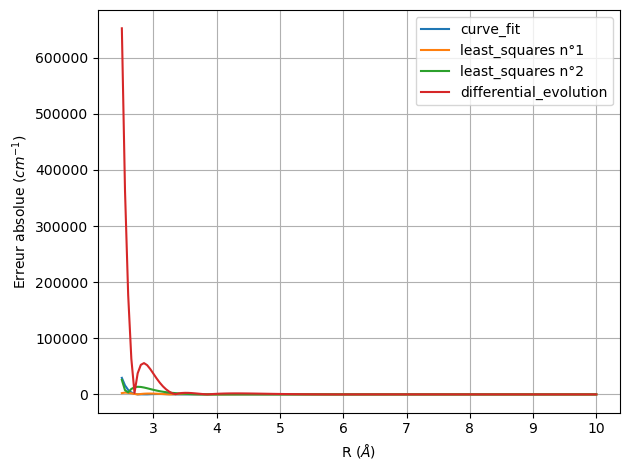
\includegraphics[width=\linewidth]{../Figures/AR-Chinois-Partiel/err_abs_Theta0.png}
    \end{subfigure}
    \begin{subfigure}{0.45\textwidth}
        \centering
        \caption{$\theta=90$°}
        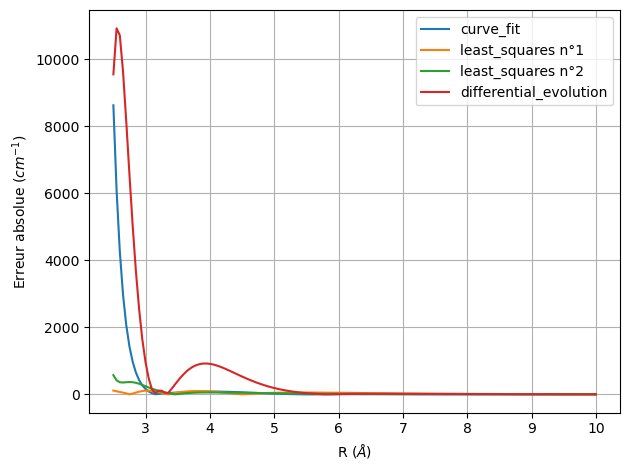
\includegraphics[width=\linewidth]{../Figures/AR-Chinois-Partiel/err_abs_Theta90.png}
    \end{subfigure}
    \begin{subfigure}{0.45\textwidth}
        \centering
        \caption{$\theta=180$°}
        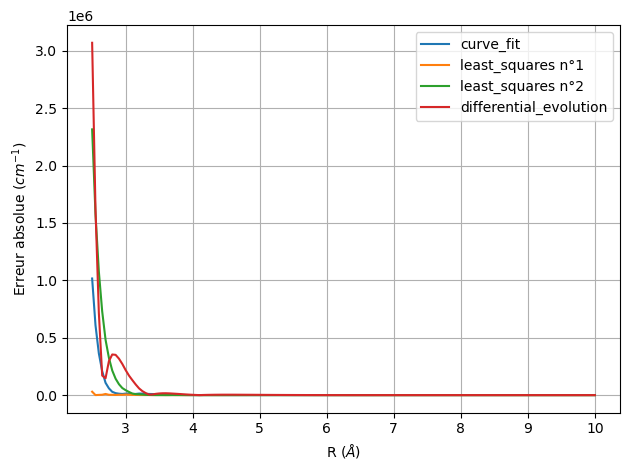
\includegraphics[width=\linewidth]{../Figures/AR-Chinois-Partiel/err_abs_Theta180.png}
    \end{subfigure}
\end{figure}
\newpage{}
\subsection{Erreur relative pour $\theta$ fixé}

\begin{figure}[h]
    \centering
    \caption{Courbes des erreurs absolues pour $\theta$ fixé}
    \begin{subfigure}{0.45\textwidth}
        \centering
        \caption{$\theta=0$°}
        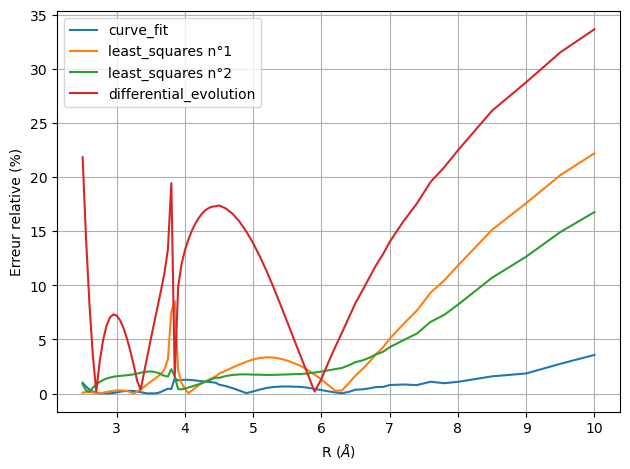
\includegraphics[width=\linewidth]{../Figures/AR-Chinois-Partiel/err_rel_Theta0.png}
    \end{subfigure}
    \begin{subfigure}{0.45\textwidth}
        \centering
        \caption{$\theta=90$°}
        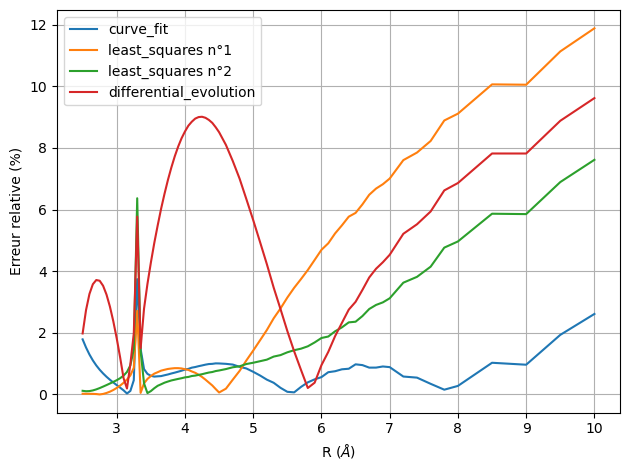
\includegraphics[width=\linewidth]{../Figures/AR-Chinois-Partiel/err_rel_Theta90.png}
    \end{subfigure}
    \begin{subfigure}{0.45\textwidth}
        \centering
        \caption{$\theta=180$°}
        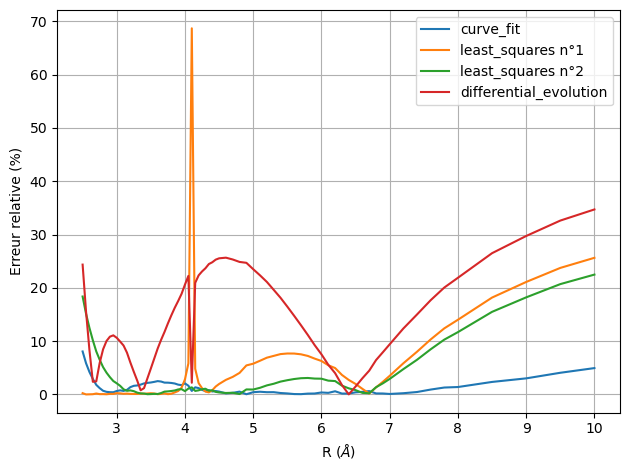
\includegraphics[width=\linewidth]{../Figures/AR-Chinois-Partiel/err_rel_Theta180.png}
    \end{subfigure}
\end{figure}

\newpage{}
\subsection{Erreur relative pour tout les $\theta$ et $R$}

\begin{figure}[h]
    \centering
    \caption{Erreur relative (\%) pour chaque $\theta$ et $R$}
    \begin{subfigure}{0.49\textwidth}
        \centering
        \caption{Méthode curve\_fit}
        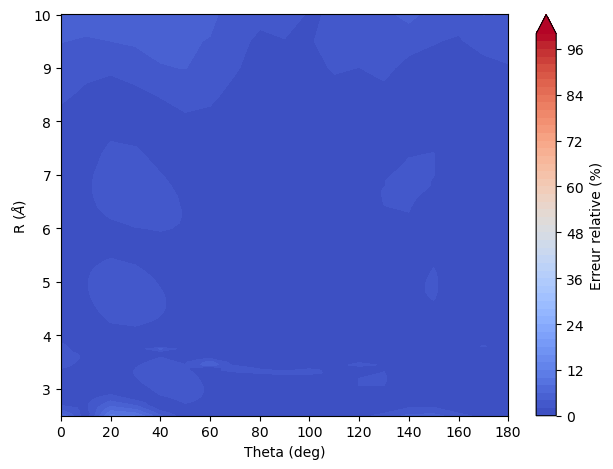
\includegraphics[width=\linewidth]{../Figures/AR-Chinois-Partiel/err_rel_all_cf.png}
    \end{subfigure}
    \begin{subfigure}{0.49\textwidth}
        \centering
        \caption{Méthode differential\_evolution}
        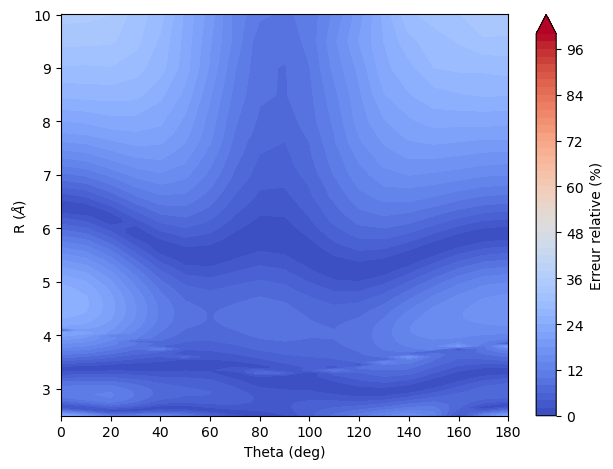
\includegraphics[width=\linewidth]{../Figures/AR-Chinois-Partiel/err_rel_all_de.png}
    \end{subfigure}
    \begin{subfigure}{0.49\textwidth}
        \centering
        \caption{Méthode least\_squares n°1}
        \label{fig:colors_ls1}
        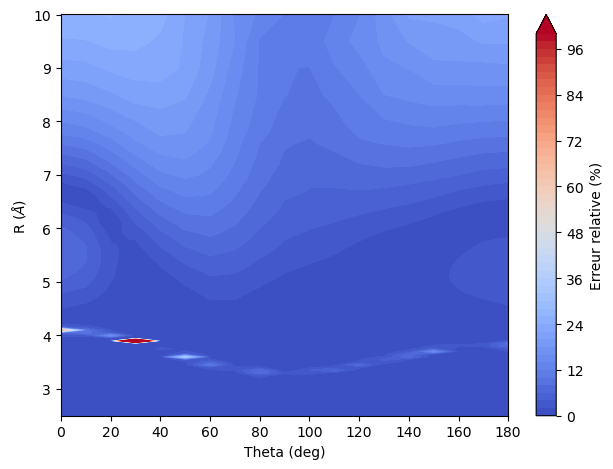
\includegraphics[width=\linewidth]{../Figures/AR-Chinois-Partiel/err_rel_all_ls1.png}
    \end{subfigure}
    \begin{subfigure}{0.49\textwidth}
        \centering
        \caption{Méthode least\_squares n°2}
        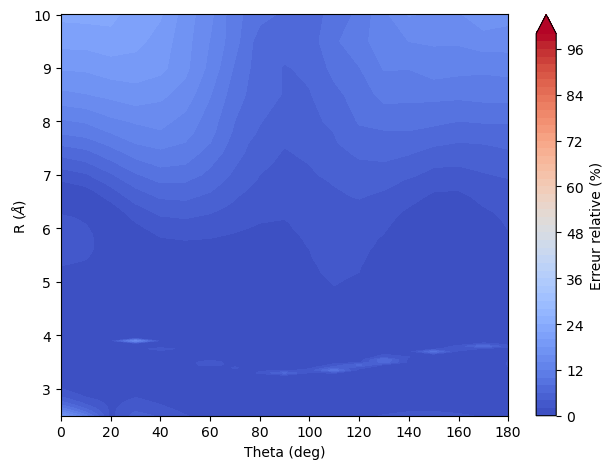
\includegraphics[width=\linewidth]{../Figures/AR-Chinois-Partiel/err_rel_all_ls2.png}
    \end{subfigure}
\end{figure}
Vous trouverez en annexe la version pour les meilleurs paramètres optimaux 
calculés à partir des données de Toczylowski (Figure~\ref{fig:err_polonais}).


\newpage{}
\section{Contour plot}

Les contours plots sont basés sur ceux données par Toczylowski dans
son article (dans le sens où on affiche les mêmes valeurs de contours).\\

Les énergies sont en cm$^{-1}$ et les R en \AA.\\

Lorsque $\theta=0$, Ar-HCN linéaire.\\

Les couleurs donnent l'erreur relative de la fonction V (de \textbf{0\% à 50\%}) pour les 
paramètres correspondant par rapport aux données ab-initio de Liman Tian.\\


\begin{figure}[h]
    \centering
    \caption{Contour plots de $V$ pour les meilleurs paramètres calculés par méthode}
    \begin{subfigure}{0.45\textwidth}
        \centering
        \caption{Méthode curve\_fit}
        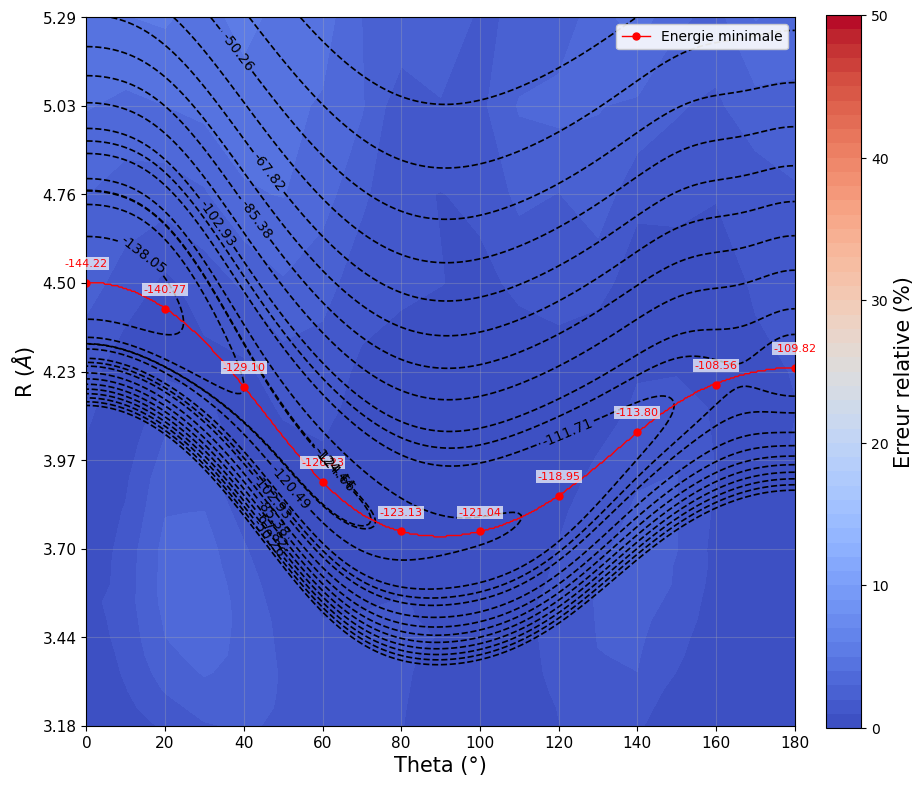
\includegraphics[width=\linewidth]{../Figures/AR-Chinois-Partiel/Contour-curve_fit.png}
    \end{subfigure}
    \begin{subfigure}{0.45\textwidth}
        \centering
        \caption{Méthode differential\_evolution}
        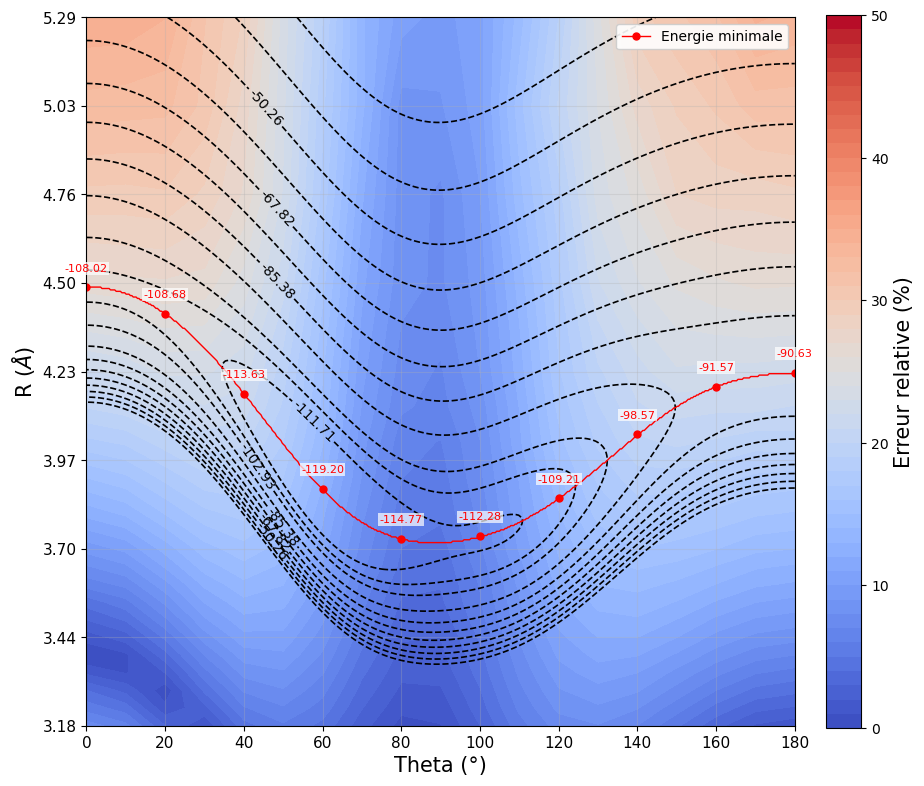
\includegraphics[width=\linewidth]{../Figures/AR-Chinois-Partiel/Contour-differential_evolution.png}
    \end{subfigure}
    \begin{subfigure}{0.45\textwidth}
        \centering
        \caption{Méthode least\_squares n°1}
        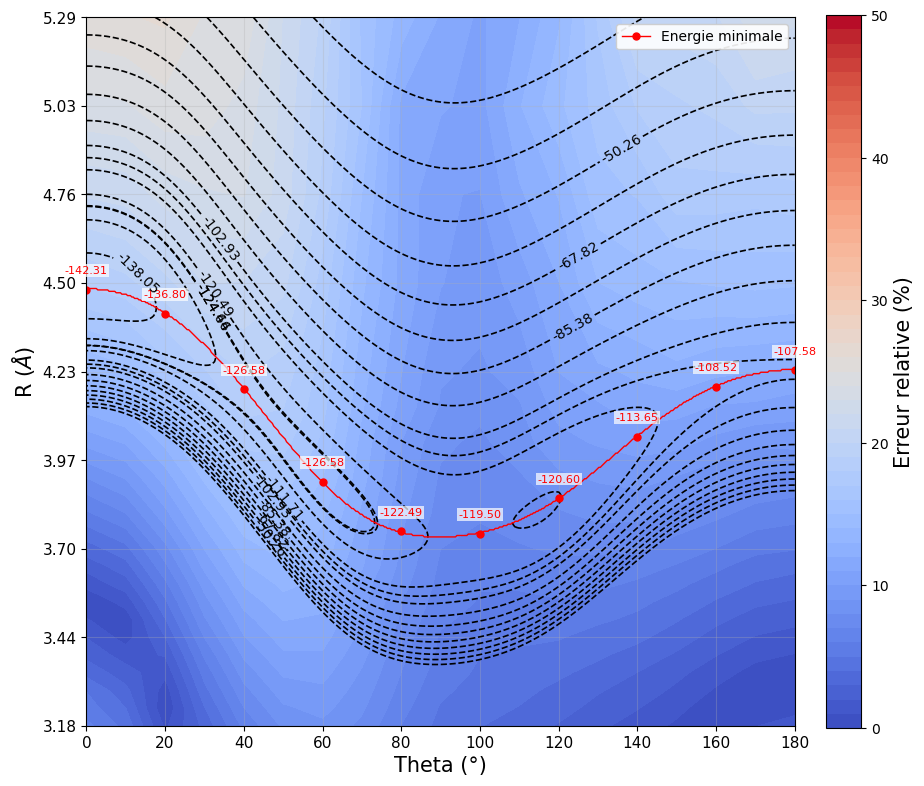
\includegraphics[width=\linewidth]{../Figures/AR-Chinois-Partiel/Contour-least_squares1.png}
    \end{subfigure}
    \begin{subfigure}{0.45\textwidth}
        \centering
        \caption{Méthode least\_squares n°2}
        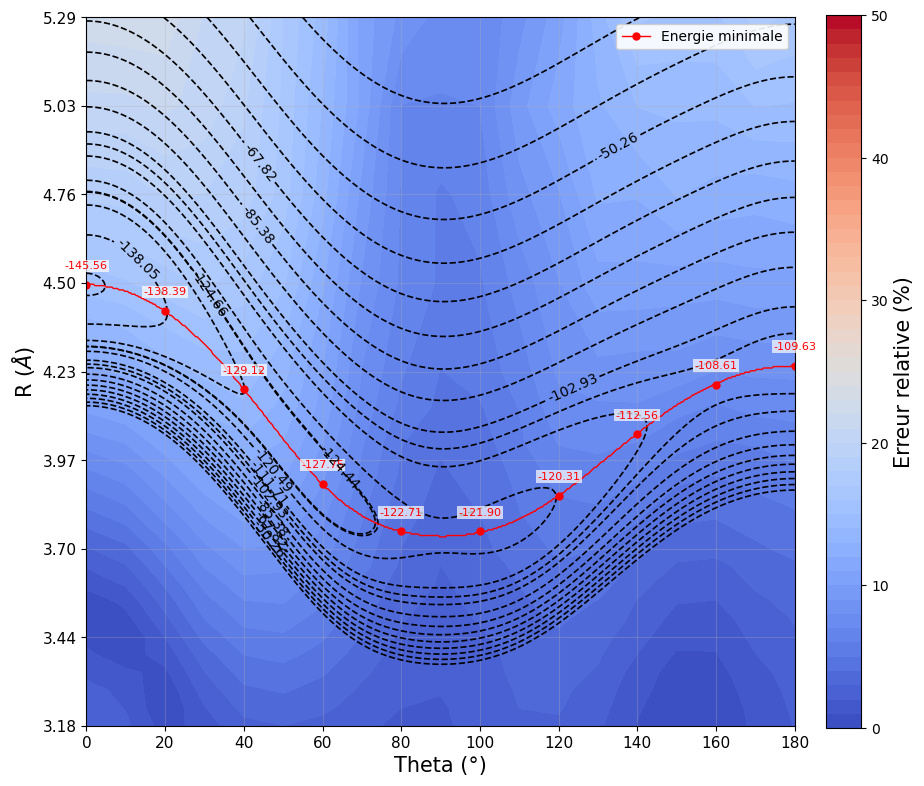
\includegraphics[width=\linewidth]{../Figures/AR-Chinois-Partiel/Contour-least_squares2.png}
    \end{subfigure}
\end{figure}

Vous trouverez en annexe la version pour les meilleurs paramètres optimaux 
calculés à partir des données de Toczylowski (Figure~\ref{fig:contour_polonais}).

\newpage{}
\section{Minimum Energy Path}

\begin{figure}[h]
    \centering
    \caption{Minimum Energy Path pour les meilleurs paramètres calculés par méthode}
    \begin{subfigure}{0.49\textwidth}
        \centering
        \caption{Méthode curve\_fit}
        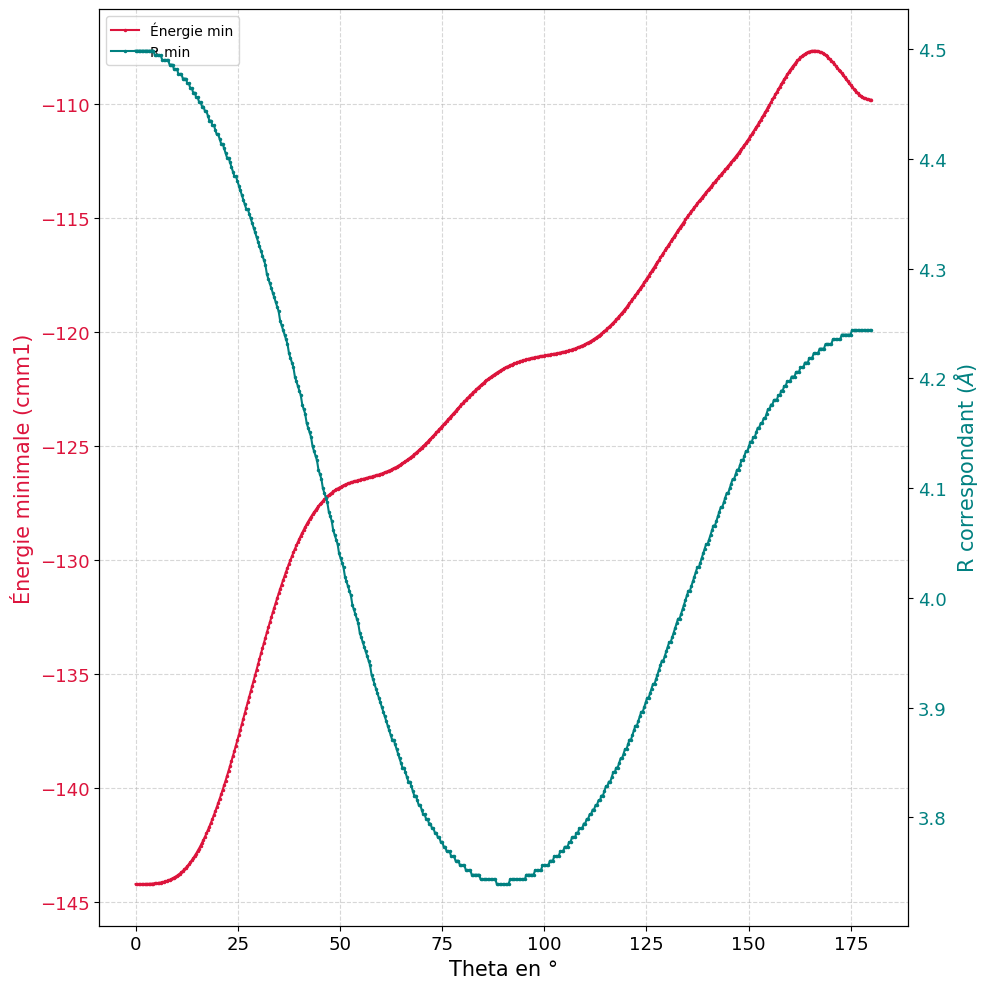
\includegraphics[width=\linewidth]{../Figures/AR-Chinois-Partiel/MEP-curve_fit.png}
    \end{subfigure}
    \begin{subfigure}{0.49\textwidth}
        \centering
        \caption{Méthode differential\_evolution}
        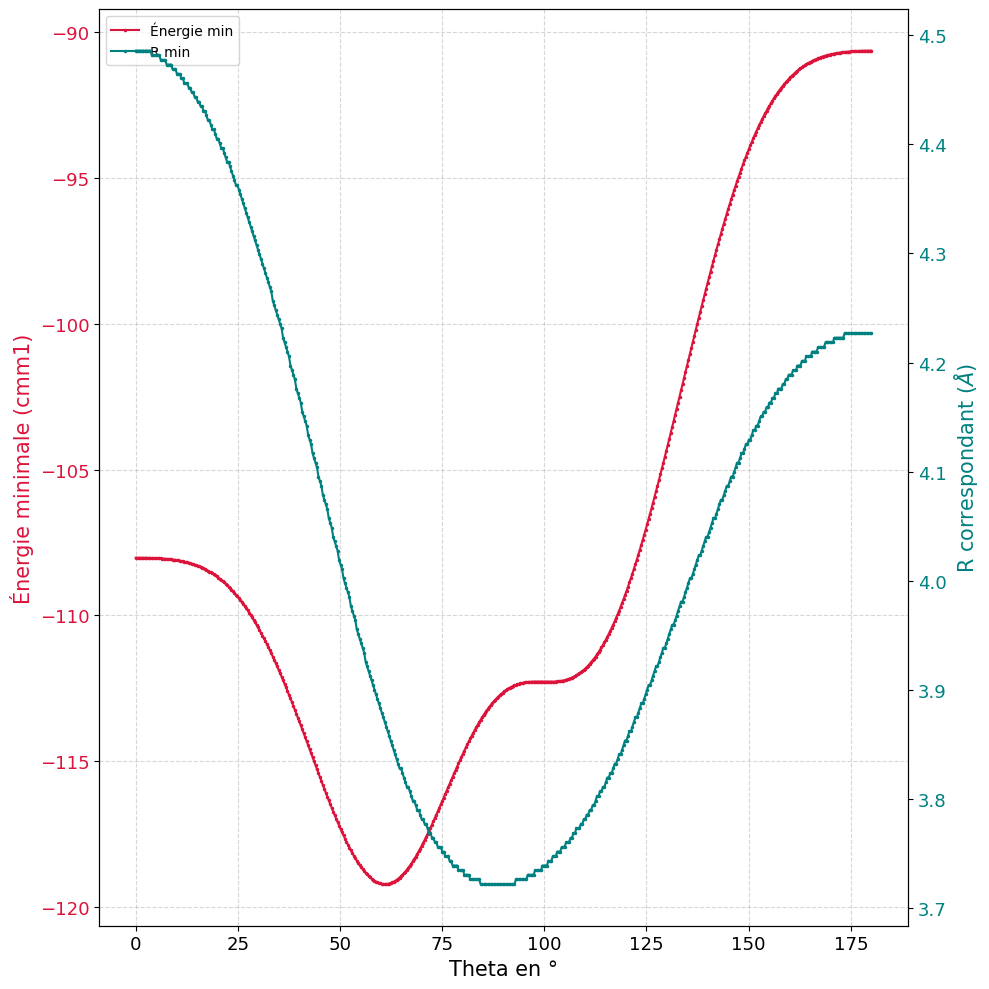
\includegraphics[width=\linewidth]{../Figures/AR-Chinois-Partiel/MEP-differential_evolution.png}
    \end{subfigure}
    \begin{subfigure}{0.49\textwidth}
        \centering
        \caption{Méthode least\_squares n°1}
        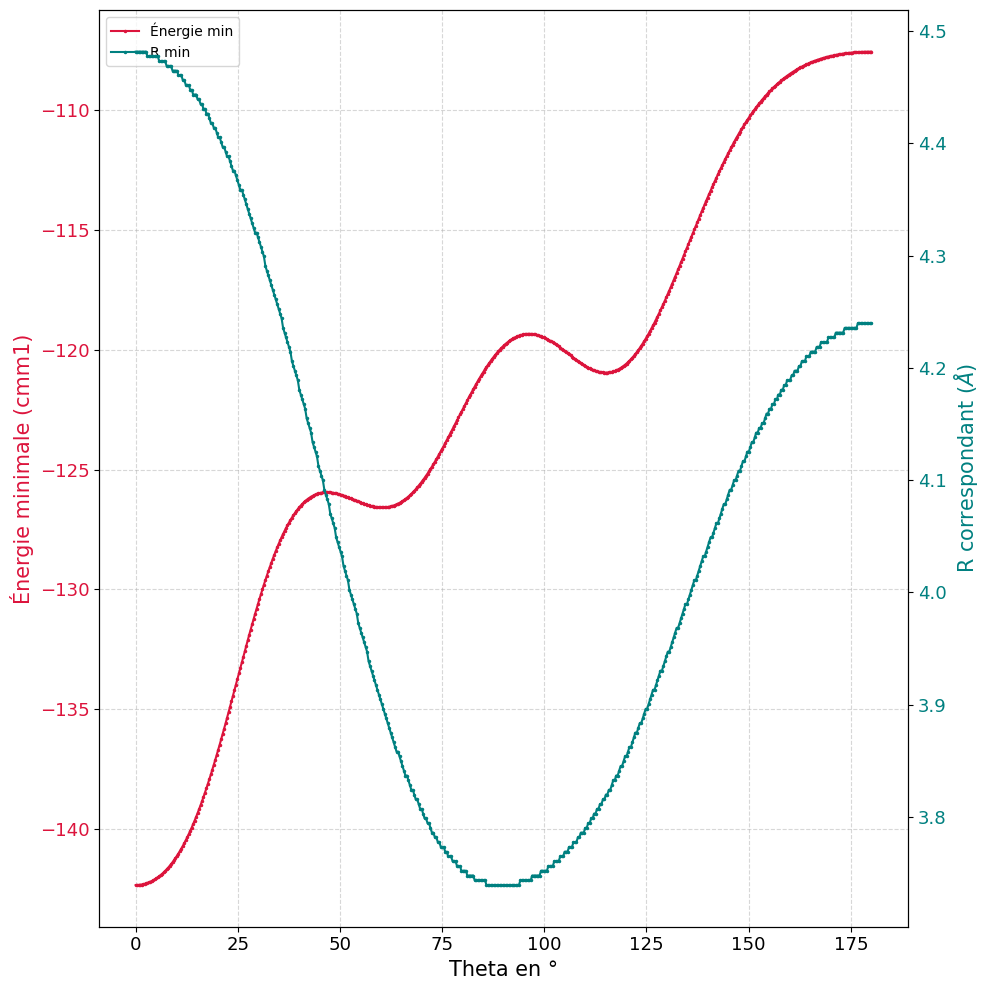
\includegraphics[width=\linewidth]{../Figures/AR-Chinois-Partiel/MEP-least_squares1.png}
    \end{subfigure}
    \begin{subfigure}{0.49\textwidth}
        \centering
        \caption{Méthode least\_squares n°2}
        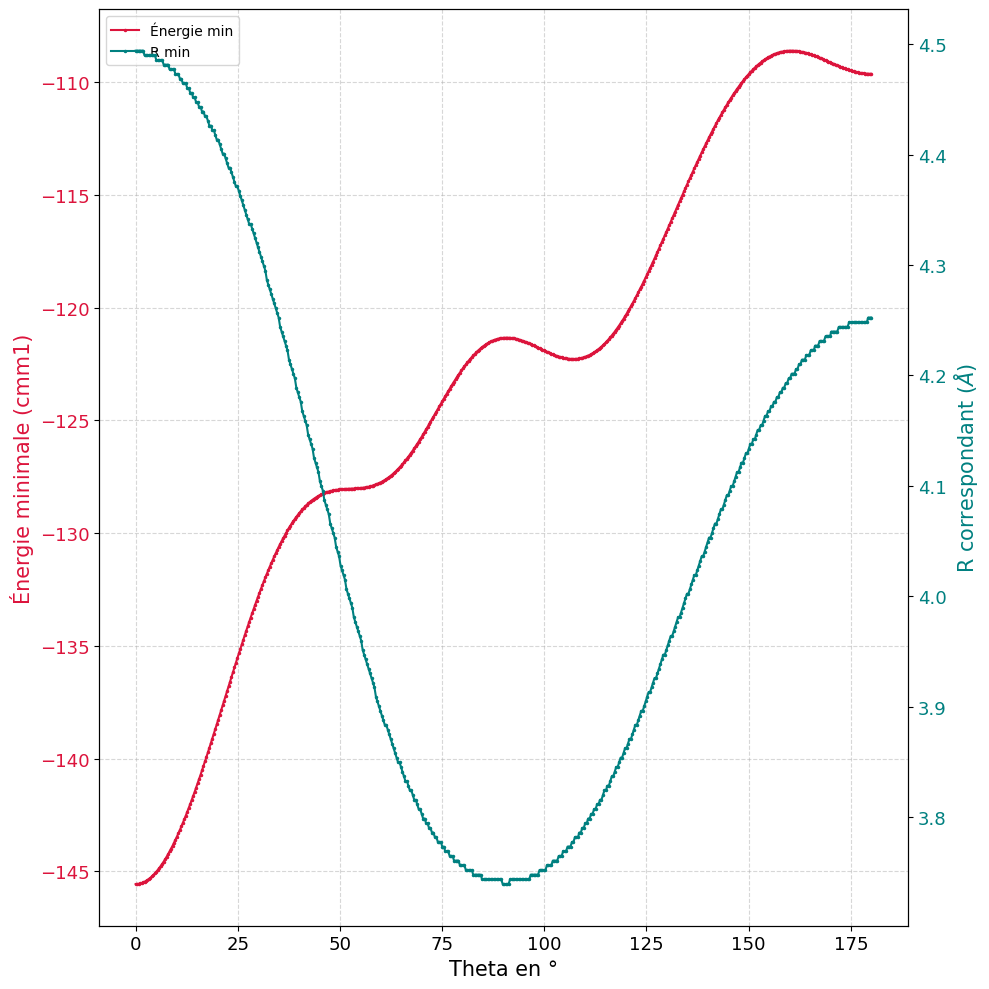
\includegraphics[width=\linewidth]{../Figures/AR-Chinois-Partiel/MEP-least_squares2.png}
    \end{subfigure}
\end{figure}
Vous trouverez en annexe la version pour les meilleurs paramètres optimaux 
calculés à partir des données de Toczylowski (Figure~\ref{fig:MEP_polonais}).

\newpage{}
\section{Courbes des énergies pour $\theta$ fixé}
\begin{figure}[h]
    \centering
    \caption{Courbes des énergies pour $\theta$ fixé}
    \begin{subfigure}{0.45\textwidth}
        \centering
        \caption{$\theta=0$°}
        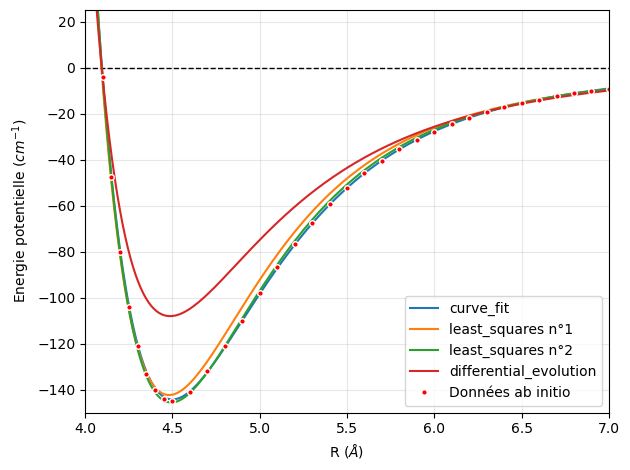
\includegraphics[width=\linewidth]{../Figures/AR-Chinois-Partiel/Courbes-Creux-Theta0.png}
    \end{subfigure}
    \begin{subfigure}{0.45\textwidth}
        \centering
        \caption{$\theta=90$°}
        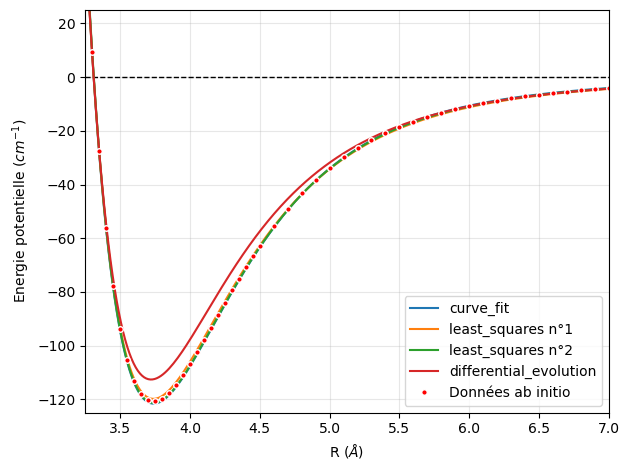
\includegraphics[width=\linewidth]{../Figures/AR-Chinois-Partiel/Courbes-Creux-Theta90.png}
    \end{subfigure}
    \begin{subfigure}{0.45\textwidth}
        \centering
        \caption{$\theta=180$°}
        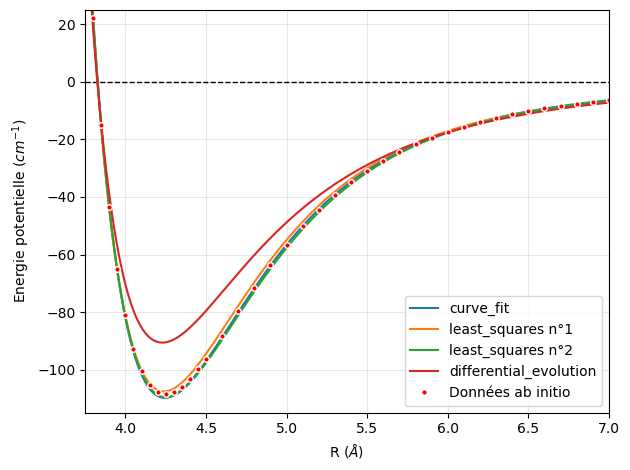
\includegraphics[width=\linewidth]{../Figures/AR-Chinois-Partiel/Courbes-Creux-Theta180.png}
    \end{subfigure}
\end{figure}

\newpage{}
\section{Courbes des énergies pour R fixé}
\begin{figure}[h]
    \centering
    \caption{Courbes des énergies pour $R$ fixé}
    \begin{subfigure}{0.45\textwidth}
        \centering
        \caption{$R=2.5$ \AA}
        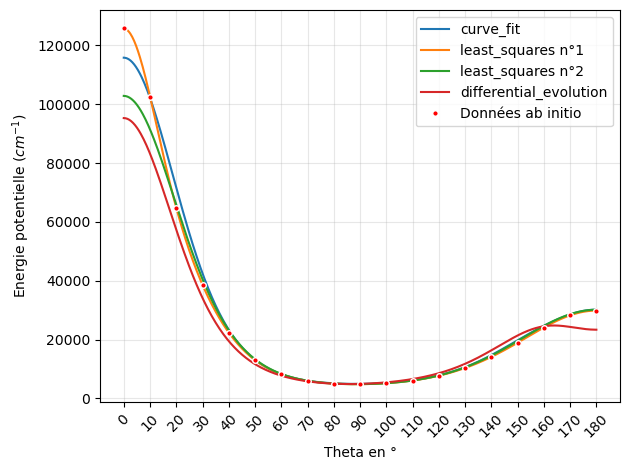
\includegraphics[width=\linewidth]{../Figures/AR-Chinois-Partiel/Courbes-R2_5.png}
    \end{subfigure}
    \begin{subfigure}{0.45\textwidth}
        \centering
        \caption{$R=4.0$ \AA}
        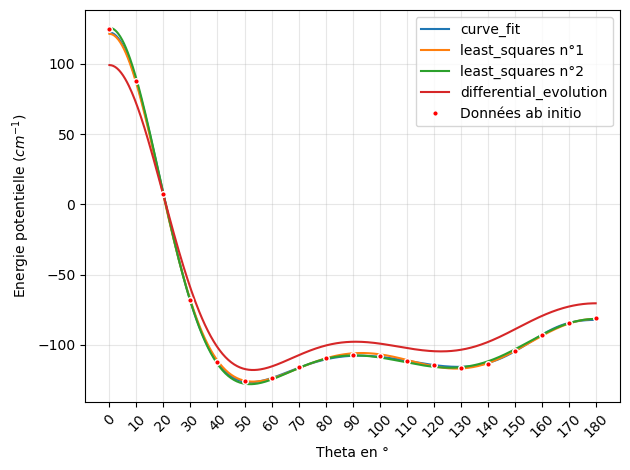
\includegraphics[width=\linewidth]{../Figures/AR-Chinois-Partiel/Courbes-R4.png}
    \end{subfigure}
    \begin{subfigure}{0.45\textwidth}
        \centering
        \caption{$R=4.5$ \AA}
        \label{fig:Courbes_R4_5}
        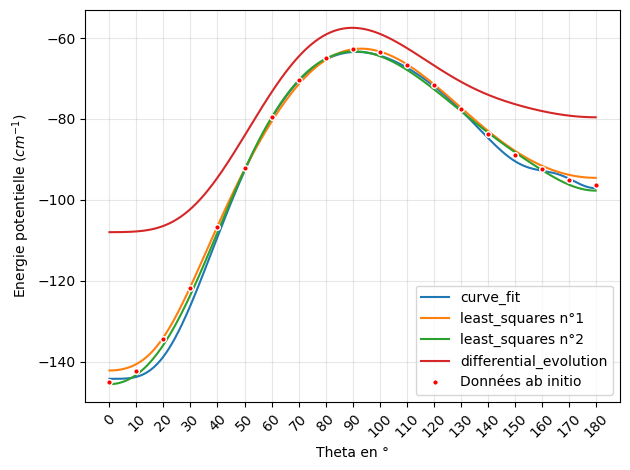
\includegraphics[width=\linewidth]{../Figures/AR-Chinois-Partiel/Courbes-R4_5.png}
    \end{subfigure}
    \begin{subfigure}{0.45\textwidth}
        \centering
        \caption{$R=10.0$ \AA}
        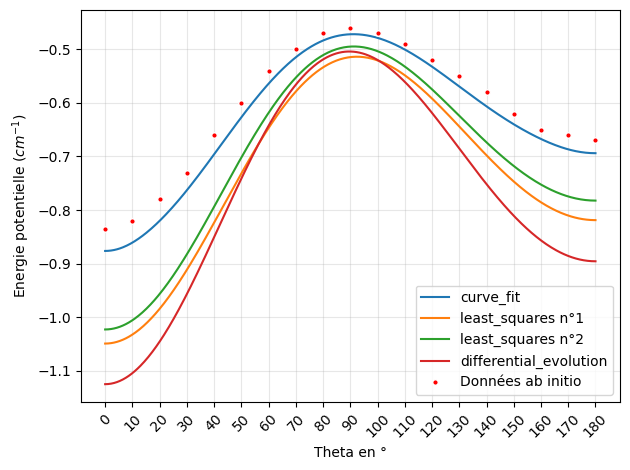
\includegraphics[width=\linewidth]{../Figures/AR-Chinois-Partiel/Courbes-R10.png}
    \end{subfigure}
\end{figure}

\section{Conclusion}

De manière globale, la méthode curve\_fit est celle qui a apporté les meilleurs paramètres. 
Ses paramètres sont ceux qui sont les plus précis pour les grandes valeurs de R mais aussi les zones
où se trouvent les énergies minimales. A noter que l'on remarque à la Figure~\ref{fig:Courbes_R4_5} 
entre $\theta=140$° et $\theta=180$° une légère oscillation.\\

Les paramètres calculés à partir de least\_squares n°1 sont "meilleurs" pour $2.5 \leq R \leq 3.25$ \AA. 
La tache rouge que l'on observe à la Figure~\ref{fig:colors_ls1} est simplement
dûe à une énergie très proche de 0, ainsi une très faible variation parait énorme voir Figure~\ref{fig:theta30}

Les erreurs données par R², RMSE et MAE font pencher vers les paramètres calculés avec \textbf{least\_squares n°1} 
mais les différents graphes montrent que \textbf{curve\_fit} et  \textbf{least\_squares n°2} sont aussi
très bons.

%--------------------------------------------------
\newpage{}
\appendix

\section{Figures complémentaires}
\begin{figure}[h]
  \caption{Erreur relative par rapport aux données de Liman Tian avec les meilleurs paramètres calculés
  à partir des données ab-initio de Toczylowski}
  \label{fig:err_polonais}
  \begin{center}
    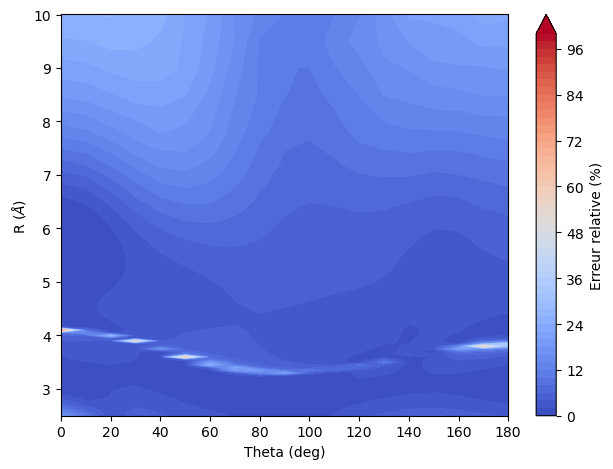
\includegraphics[width=0.49\textwidth]{../Figures/AR-Chinois-Partiel/err_rel_all_polonais.png}
  \end{center}
\end{figure}

\begin{figure}[h]
  \caption{Contour plots de $V$ pour les meilleurs paramètres calculés à partir
  des données ab-initio de Toczylowski - Erreur relative en fonction des données
  de Liman Tian}
  \label{fig:contour_polonais}
  \begin{center}
    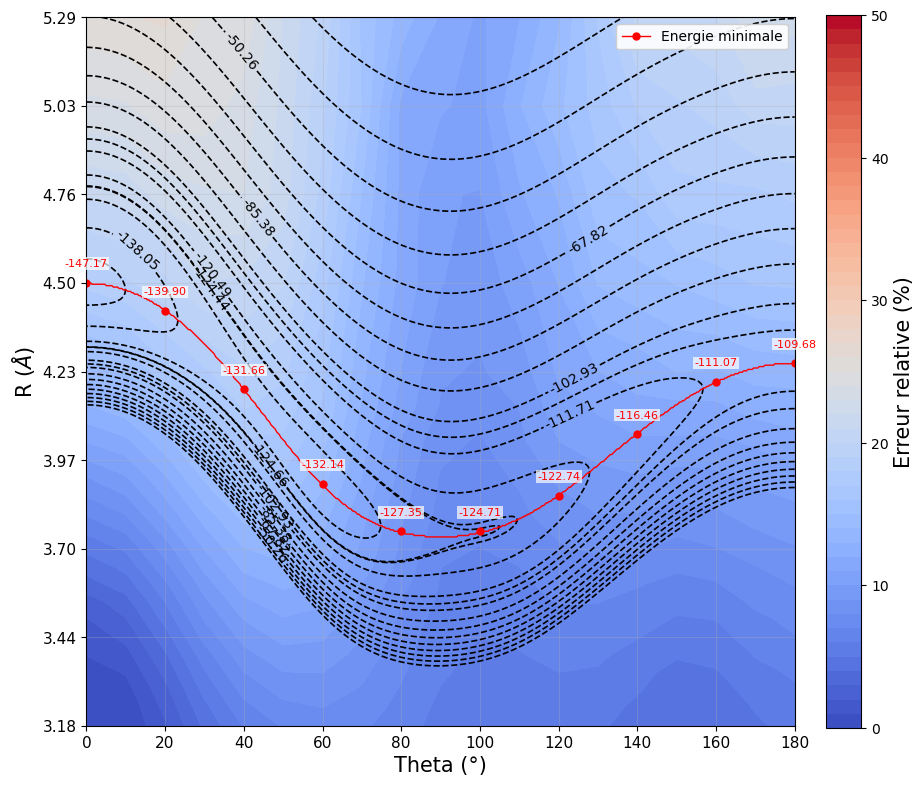
\includegraphics[width=0.49\textwidth]{../Figures/AR-Chinois-Partiel/Contour-polonais.png}
  \end{center}
\end{figure}

\begin{figure}[h]
  \caption{Minimum Energy Path pour les meilleurs paramètres calculés à partir
  des données ab-initio de Toczylowski}
  \label{fig:MEP_polonais}
  \begin{center}
    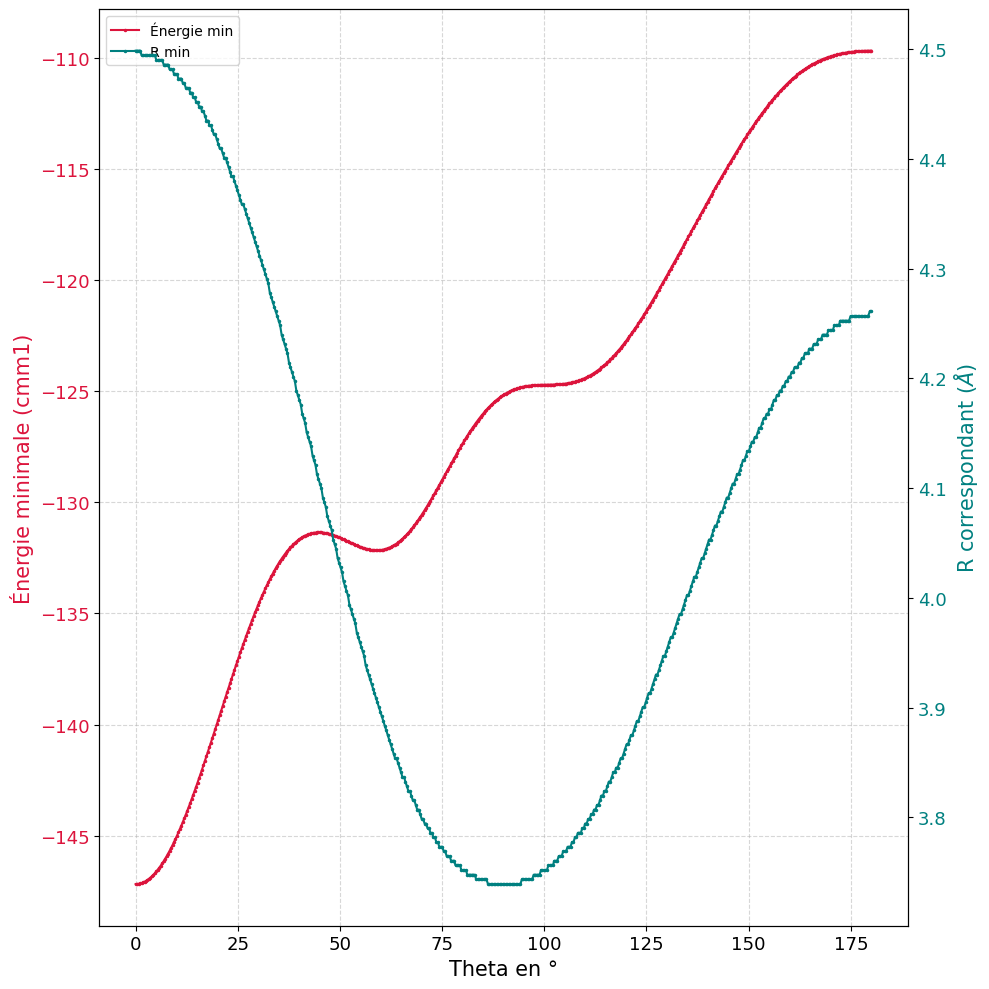
\includegraphics[width=0.49\textwidth]{../Figures/AR-Chinois-Partiel/MEP-polonais.png}
  \end{center}
\end{figure} 

\begin{figure}[h]
  \caption{Courbes des énergies pour $\theta=30$°}\label{fig:theta30}
  \begin{center}
    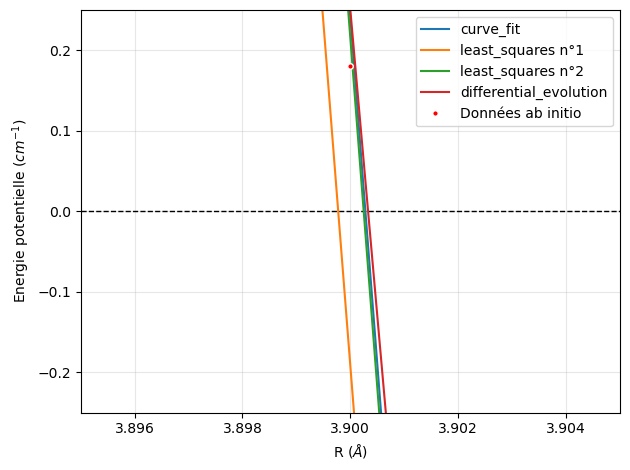
\includegraphics[width=0.55\textwidth]{../Figures/AR-Chinois-Partiel/Courbes-Creux-Theta30.png}
  \end{center}
\end{figure}


%--------------------------------------------------
\bibliographystyle{plain}
\bibliography{references}

\end{document}
